%%
%% UW CBE Thesis: chapterthreename/chapterthreename.tex
%% Written by Ankur Gupta, Sep 1, 2013
%% Departament of Chemical and Biological Engineering
%% University of Wisconsin-Madison
%% Copyright (c) Ankur Gupta, 2014
%%
%% License: GPL v3. See LICENSE.
%%

% This is Chapter 3. You're doing well.
% Keep going.
\chapter{Chapter Three Title}
\label{chap:chapterthreename}
\doublespacing
\index{famous kingdoms}

\section{Famous Kingdons}

\subsection{Seven Kingdoms of Westeros}

\begin{table}
\centering
\caption{Seven Kingdoms of Westeros and their capitals}
\begin{tabular}{lc}
\toprule
Kingdom & Capital \\
\midrule
The North  & Winterfell \\
Iron Islands & Pyke \\
Vale of Arryn & Eyrie \\
The Westerlands & Casterly Rock \\
The Reach & Highgarden \\
The Stormlands & Storm's End \\
Dorne & Sunspear \\
\bottomrule
\end{tabular}
\end{table}

\section{Casterly Rock}
\index{Casterly Rock}
According to Wikipedia, Casterly Rock was inspired by the Rock of Gibralter\index{Rock of Gibralter}.
Figure~\ref{fig:rock} shows a picture of the Rock of Gibralter, taken from Wikipedia.

\begin{figure}
\centering
\caption{Rock of Gibralter}
\label{fig:rock}
% Remember you need to give the path with respect to the location of thesis.tex
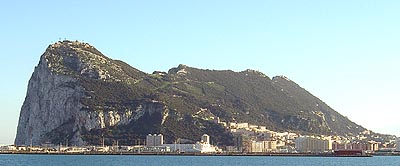
\includegraphics[width=\textwidth]{chapterthreename/figures/Rock_of_Gibraltar_northwest.jpg}
\tiny Source: Wikipedia
\end{figure}





